\Opensolutionfile{ans}[ans/G12D1TN]
% ===================================================================
\begin{ex}
	Hãy tìm ý \textbf{không đúng} với mô hình động học phân tử.
	\choice
	{\True Tốc độ chuyển động của các phân tử cấu tạo nên vật càng lớn thì thể tích của vật càng lớn}
	{Các chất được cấu tạo từ các hạt riêng biệt là phân tử}
	{Các phân tử chuyển động không ngừng}
	{Giữa các phân tử có lực tương tác gọi là lực liên kết phân tử}
	\loigiai{}
\end{ex}

% ===================================================================
\begin{ex}
	Câu nào sau đây nói về nội năng là \textbf{không đúng}?
	\choice
	{Nội năng là một dạng năng lượng}
	{Nội năng có thể chuyển hoá thành năng lượng khác}
	{\True Nội năng là nhiệt lượng}
	{Nội năng của một vật có thể tăng lên hoặc giảm đi}
	\loigiai{}
\end{ex}
% ===================================================================
\begin{ex}
	Hiện tượng vào mùa đông ở các nước vùng băng tuyết thường xảy ra sự cố vỡ đường ống nước là do
	\choice
	{tuyết rơi nhiều đè nặng thành ống}
	{\True thể tích nước khi đông đặc tăng lên gây ra áp lực lớn lên thành ống}
	{trời lạnh làm đường ống bị cứng dòn và rạn nứt}
	{các phương án đưa ra đều sai}
	\loigiai{}
\end{ex}

% ===================================================================
\begin{ex}
	Nội năng của một vật phụ thuộc vào
	\choice
	{Nhiệt độ, áp suất và khối lượng}
	{Nhiệt độ và áp suất}
	{\True Nhiệt độ và thể tích}
	{Nhiệt độ, áp suất và thể tích}
	\loigiai{}
\end{ex}
% ===================================================================
\begin{ex}
	Đặc điểm nào sau đây là của sự bay hơi?
	\choice
	{\True Xảy ra ở bất kì nhiệt độ nào của chất lỏng}
	{Chỉ xảy ra trong lòng chất lỏng}
	{Xảy ra với tốc độ như nhau ở mọi nhiệt độ}
	{Chỉ xảy ra đối với một số ít chất lỏng}
	\loigiai{}
\end{ex}

% ===================================================================
\begin{ex}
	Nhiệt độ nóng chảy riêng của vật rắn phụ thuộc vào những yếu tố nào?
	\choice
	{Phụ thuộc vào nhiệt độ của vật rắn và áp suất ngoài}
	{\True Phụ thuộc bản chất của vật rắn}
	{Phụ thuộc bản chất và nhiệt độ của vật rắn}
	{Phụ thuộc bản chất và nhiệt độ của vật rắn, đồng thời phụ thuộc áp suất ngoài}
	\loigiai{}
\end{ex}

% ===================================================================
\begin{ex}
Quy ước về dấu nào sau đây phù hợp với công thức định luật I nhiệt động lực học $\Delta U=A+Q$?	
	\choice
	{Vật nhận công: $A<0$; vật nhận nhiệt: $Q<0$}
	{\True Vật nhận công: $A>0$; vật nhận nhiệt: $Q>0$}
	{Vật thực hiện công: $A<0$; vật truyền nhiệt: $Q>0$}
	{Vật thực hiện công: $A>0$; vật truyền nhiệt: $Q<0$}
	\loigiai{}
\end{ex}
% ===================================================================
\begin{ex}
Khối khí thực hiện công trong quá trình nào sau đây?	
	\choice
	{\True Nhiệt lượng khối khí nhận được lớn hơn độ tăng nội năng của khí}
	{Nhiệt lượng khối khí nhận được nhỏ hơn độ tăng nội năng của khí}
	{Nhiệt lượng khối khí nhận được bằng độ tăng nội năng của khí}
	{Nhiệt lượng khối khí toả ra lớn hơn độ giảm nội năng của khí}
	\loigiai{}
\end{ex}
% ===================================================================
\begin{ex}
	Câu nào sau đây nói về sự truyền nhiệt là \textbf{không đúng}?
	\choice
	{Nhiệt không thể tự truyền từ vật lạnh hơn sang vật nóng hơn}
	{Nhiệt có thể tự truyền từ vật nóng hơn sang vật lạnh hơn}
	{Nhiệt có thể truyền từ vật lạnh hơn sang vật nóng hơn}
	{\True Nhiệt có thể tự truyền giữa hai vật có cùng nhiệt độ}
	\loigiai{Nhiệt không thể tự truyền nếu hai vật không có sự chênh lệch nhiệt độ.\\
	Câu C đúng vì nhiệt không thể tự truyền từ vật lạnh sang vật nóng nhưng nếu có bơm nhiệt (như máy lạnh) thì có thể được.}
\end{ex}
% ===================================================================
\begin{ex}
	Trường hợp nào dưới đây làm biến đổi nội năng không do thực hiện công?
	\choice
	{\True Đun nước bằng bếp}
	{Một viên bi bằng thép rơi xuống đất mềm}
	{Cọ xát hai vật với nhau}
	{Nén khí trong xi lanh}
	\loigiai{}
\end{ex}
% ===================================================================
\begin{ex}
	Nhiệt độ bề mặt của Mặt Trời là $\SI{5772}{\kelvin}$. Nhiệt độ bề mặt của Mặt Trời theo nhiệt giai Celsius là bao nhiêu?
	\choice
	{$\SI{6045}{\celsius}$}
	{$\SI{3189}{\celsius}$}
	{\True $\SI{5499}{\celsius}$}
	{$\SI{6009}{\celsius}$}
	\loigiai{
	$$t\left(\si{\celsius}\right)=T\left(\si{\kelvin}\right)-273=\SI{5499}{\celsius}.$$}
\end{ex}
% ===================================================================
\begin{ex}
	Nhiệt độ ở Paris ngày 07/06/2024 là $\SI{71}{\degree F}$. Nhiệt độ của ngày hôm đó nếu tính theo thang Celsius sẽ là
	\choice
	{\True $\SI{22}{\celsius}$}
	{$\SI{39}{\celsius}$}
	{$\SI{28}{\celsius}$}
	{$\SI{32}{\celsius}$}
	\loigiai{
$$t\left(\si{\celsius}\right)=\dfrac{t\left(\si{\degree F}\right)-32}{1,8}\approx\SI{22}{\celsius}.$$	
}
\end{ex}
% ===================================================================
\begin{ex}
	Người ta thực hiện công $\SI{100}{\joule}$ để nén khí trong một cylanh. Tính độ biến thiên nội năng của khí, biết khí truyền ra môi trường xung quanh nhiệt lượng $\SI{20}{\joule}$.
	\choice
	{$\SI{120}{\joule}$}
	{\True $\SI{80}{\joule}$}
	{$\SI{100}{\joule}$}
	{$\SI{60}{\joule}$}
	\loigiai{
Khí nhận công và truyền nhiệt nên: $A=\SI{100}{\joule}$; $Q=\SI{-20}{\joule}$.\\
Độ biến thiên nội năng của khí:
$$\Delta U=Q+A=\SI{80}{\joule}.$$	
}
\end{ex}
% ===================================================================
\begin{ex}
	Cung cấp cho vật một công $\SI{200}{\joule}$ nhưng nhiệt lượng bị thất thoát ra môi trường xung quanh là $\SI{120}{\joule}$. Nội năng của vật 
	\choice
	{\True tăng $\SI{80}{\joule}$}
	{giảm $\SI{80}{\joule}$}
	{không thay đổi}
	{giảm $\SI{320}{\joule}$}
	\loigiai{
Vật nhận công và toả nhiệt nên: $A=\SI{200}{\joule}$; $Q=\SI{-120}{\joule}$.\\
Độ biến thiên nội năng của vật:
$$\Delta U=Q+A=\SI{80}{\joule}.$$	
}
\end{ex}
% ===================================================================
\begin{ex}
Khi hai vật có nhiệt độ khác nhau tiếp xúc với nhau thì xảy ra quá trình truyền nhiệt. Quá trình này làm thay đổ	
	\choice
	{khối lượng của các vật}
	{trọng lượng của các vật}
	{\True nội năng của các vật}
	{nhiệt dung riêng của các vật}
	\loigiai{}
\end{ex}
% ===================================================================
\begin{ex}
Nhiệt dung riêng của đồng lớn hơn nhiệt dung riêng của chì. Vì vậy, để tăng nhiệt độ của $\SI{3}{\kilogram}$ đồng và $\SI{3}{\kilogram}$ chì thêm $\SI{15}{\celsius}$ thì	
	\choice
	{Khối chì cần nhiều nhiệt lượng hơn khối đồng}
	{\True Khối đồng cần nhiều nhiệt lượng hơn khối chì}
	{Hai khối đều cần nhiệt lượng như nhau}
	{Không khẳng định được}
	\loigiai{}
\end{ex}
% ===================================================================
\begin{ex}
Ba chất lỏng A. B. C đang ở nhiệt độ $t_\text{A}$, $t_\text{B}$, $t_\text{C}$ với $t_\text{A}<t_\text{B}<t_\text{C}$ được trộn lẫn với nhau. Chất lỏng nào tỏa nhiệt, chất lỏng nào thu nhiệt?	
	\choice
	{A tỏa nhiệt, B và C thu nhiệt}
	{A và B tỏa nhiệt, C thu nhiệt}
	{C tỏa nhiệt, A và B thu nhiệt}
	{\True Chỉ khẳng định được sau khi tính được nhiệt độ khi cân bằng}
	\loigiai{}
\end{ex}

% ===================================================================
\begin{ex}
	$\SI{100}{\gram}$ chì được truyền nhiệt lượng $\SI{260}{\joule}$, thì tăng nhiệt độ từ $\SI{15}{\celsius}$ đến $\SI{35}{\celsius}$. Nhiệt dung riêng của chì là
	\choice
	{\True $\SI{130}{\joule/\left(\kilogram\cdot\kelvin\right)}$}
	{$\SI{26}{\joule/\left(\kilogram\cdot\kelvin\right)}$}
	{$\SI{130}{\kilo\joule/\left(\kilogram\cdot\kelvin\right)}$}
	{$\SI{260}{\kilo\joule/\left(\kilogram\cdot\kelvin\right)}$}
	\loigiai{$$c=\dfrac{Q}{m\Delta T}=\dfrac{\SI{260}{\joule}}{\left(\SI{0.1}{\kilogram}\right)\cdot\left(\SI{20}{\kelvin}\right)}=\SI{130}{\joule/\left(\kilogram\cdot\kelvin\right)}.$$}
\end{ex}
% ===================================================================
\begin{ex}
	Tính nhiệt lượng cần cung cấp để đun nóng $\SI{5}{\kilogram}$ nước từ nhiệt độ $\SI{20}{\celsius}$ lên $\SI{100}{\celsius}$. Biết nhiệt dung riêng của nước là $\SI{4.18}{\kilo\joule/\left(\kilogram\cdot\kelvin\right)}$
	\choice
	{$\SI{1267E3}{\joule}$}
	{\True $\SI{1672E3}{\joule}$}
	{$\SI{3344E3}{\joule}$}
	{$\SI{836E3}{\joule}$}
	\loigiai{$$Q=mc\Delta T=\left(\SI{5}{\kilogram}\right)\cdot\left(\SI{4.18E3}{\joule/\left(\kilogram\cdot\kelvin\right)}\right)\cdot\left(\SI{80}{\kelvin}\right)=\SI{1672E3}{\joule}.$$}
\end{ex}
% ===================================================================
\begin{ex}
	Tính nhiệt lượng do miếng sắt khối lượng $\SI{2}{\kilogram}$ toả ra khi hạ nhiệt độ từ $\SI{500}{\celsius}$ xuống còn $\SI{40}{\celsius}$. Biết nhiệt dung riêng của sắt là $\SI{478}{\joule/\left(\kilogram\cdot\kelvin\right)}$
	\choice
	{$\SI{219880}{\joule}$}
	{\True $\SI{439760}{\joule}$}
	{$\SI{879520}{\joule}$}
	{$\SI{109940}{\joule}$}
	\loigiai{
Nhiệt lượng miếng sắt toả ra:
$$Q=mc\left(t_1-t_2\right)=\SI{439760}{\joule}.$$	
}
\end{ex}
% ===================================================================
\begin{ex}
	Biết nhiệt nóng chảy riêng của nước đá là $\SI{3.34E5}{\joule/\kilogram}$. Người ta cung cấp nhiệt lượng $\SI{5.01E5}{\joule}$ có thể làm nóng chảy hoàn toàn bao nhiêu $\si{\kilogram}$ nước đá?
	\choice
	{$\SI{16.7}{\kilogram}$}
	{\True $\SI{1.5}{\kilogram}$}
	{$\SI{8.35}{\kilogram}$}
	{$\SI{0.668}{\kilogram}$}
	\loigiai{Khối lượng nước đá nóng chảy hoàn toàn:
	$$m=\dfrac{Q}{\lambda}=\SI{1.5}{\kilogram}.$$}
\end{ex}

% ===================================================================
\begin{ex}
	Một viên đạn bằng bạc đang bay với tốc độ $\SI{200}{\meter/\second}$ thì va chạm vào một bức tường gỗ và nằm yên trong bức tường. Nhiệt dung riêng của bạc là $\SI{234}{\joule/\left(\kilogram\cdot\kelvin\right)}$. Nếu coi viên đạn không trao đổi nhiệt với bên ngoài thì nhiệt độ của viên đạn sẽ tăng thêm bao nhiêu độ?
	\choice
	{$\SI{58}{\celsius}$}
	{$\SI{171}{\celsius}$}
	{\True $\SI{85}{\celsius}$}
	{$\SI{250}{\celsius}$}
	\loigiai{
Áp dụng định luật bảo toàn và chuyển hoá năng lượng:
$$\dfrac{1}{2}mv^2=mc\Delta t\Rightarrow \Delta t=\dfrac{v^2}{2c}\approx\SI{85}{\celsius}.$$	
}
\end{ex}
% ===================================================================
\begin{ex}
	Đầu thép của một búa máy có khối lượng $\SI{15}{\kilogram}$ nóng lên thêm $\SI{20}{\celsius}$ sau 1,6 phút hoạt động. Biết rằng chỉ có $\SI{40}{\percent}$ cơ năng của búa máy chuyển thành nhiệt năng của đầu búa. Công và công suất của búa máy có giá trị là bao nhiêu? Biết nhiệt dung riêng của thép là $\SI{460}{\joule/\left(\kilogram\cdot\kelvin\right)}$.
	\begin{center}
	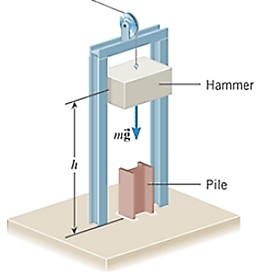
\includegraphics[width=0.35\linewidth]{../figs/G12-D1-1}
	\end{center}
	\choice
	{\True $A=\SI{345}{\kilo\joule}$; $\calP=\SI{3593.75}{\watt}$}
	{$A=\SI{345}{\kilo\joule}$; $\calP=\SI{1953.75}{\watt}$}
	{$A=\SI{345}{\joule}$; $\calP=\SI{15.9375}{\watt}$}
	{$A=\SI{345}{\kilo\joule}$; $\calP=\SI{19.5375}{\watt}$}
	\loigiai{
Công của búa máy:
$$A=\dfrac{mc\Delta t}{H}=\SI{345}{\kilo\joule}.$$
Công suất của búa máy:
$$\calP=\dfrac{A}{t}=\SI{3593.75}{\watt}.$$	
}
\end{ex}
% ===================================================================
\begin{ex}
Tính nhiệt lượng toả ra khi $\SI{4}{\kilogram}$ hơi nước ở $\SI{100}{\celsius}	$ ngưng tụ thành nước ở $\SI{22}{\celsius}$. Nước có nhiệt dung riêng $c=\SI{4180}{\joule/\left(\kilogram\cdot\kelvin\right)}$ và nhiệt hoá hơi riêng $L=\SI{2.3E6}{\joule/\kilogram}$. Chọn đáp án \textbf{đúng}.
	\choice
	{$\SI{11504160}{\joule}$}
	{$\SI{12504160}{\joule}$}
	{\True $\SI{10504160}{\joule}$}
	{$\SI{13504160}{\joule}$}
	\loigiai{
Nhiệt lượng do hơi nước toả ra để ngưng tụ thành nước ở $\SI{22}{\celsius}$:
$$Q=mL+mc\Delta t=\SI{10504160}{\joule}.$$
}
\end{ex}
% ===================================================================
\begin{ex}
Một hòn bi thép có trọng lượng $\SI{0.5}{\newton}$ rơi từ độ cao $\SI{2}{\meter}$ xuống một tấm đá rồi nảy lên tới độ cao $\SI{1.4}{\meter}$. Lượng cơ năng đã chuyển hoá thành nội năng của bi và tấm đá là
	\choice
	{$\SI{0.6}{\joule}$}
	{$\SI{0.9}{\joule}$}
	{$\SI{0.5}{\joule}$}
	{\True $\SI{0.3}{\joule}$}
	\loigiai{
Phần cơ năng đã chuyển hoá thành nội năng:
$$\Delta U=W-W'=P\left(h-h'\right)=\SI{0.3}{\joule}.$$
}
\end{ex}

% ===================================================================
\begin{ex}
Thả một quả cầu bằng nhôm có khối lượng $\SI{0.21}{\kilogram}$ được nung nóng đến $\SI{200}{\celsius}$ vào cốc đựng nước ở $\SI{30}{\celsius}$. Sau một thời gian, nhiệt độ của nước và quả cầu đều bằng $\SI{50}{\celsius}$. Biết nhiệt dung riêng của nhôm là $\SI{880}{\joule/\left(\kilogram\cdot\kelvin\right)}$, nhiệt dung riêng của nước là $\SI{4200}{\joule/\left(\kilogram\cdot\kelvin\right)}$. Khối lượng nước trong cốc là	
	\choice
	{$\SI{3.3}{\kilogram}$}
	{$\SI{7.5}{\kilogram}$}
	{$\SI{0.21}{\kilogram}$}
	{\True $\SI{0.33}{\kilogram}$}
	\loigiai{
	Áp dụng phương trình cân bằng nhiệt:
$$m_1c_1\left(t_\text{cb}-t_1\right)+m_2c_2\left(t_\text{cb}-t_2\right)=0$$
$$\Rightarrow m_2=\dfrac{m_1c_1\left(t_\text{cb}-t_1\right)}{c_2\left(t_2-t_\text{cb}\right)}=\SI{0.33}{\kilogram}.$$ }

\end{ex}
% ===================================================================
\begin{ex}
Cần cung cấp nhiệt lượng bằng bao nhiêu để làm cho $m=\SI{200}{\gram}$ nước lấy ở $t_1=\SI{10}{\celsius}$ sôi ở $t_2=\SI{100}{\celsius}$ và $\SI{10}{\percent}$ khối lượng của nó hoá hơi khi sôi. Biết nhiệt dung riêng của nước là $c=\SI{4190}{\joule/\left(
	\kilogram\cdot\kelvin\right)}$ và nhiệt hoá hơi của nước là $L=\SI{2.26E6}{\joule/\kilogram}$. Chọn đáp án \textbf{đúng}.
	\choice
	{$\SI{129525}{\joule}$}
	{$\SI{110610}{\joule}$}
	{\True $\SI{120620}{\joule}$}
	{$\SI{130610}{\joule}$}
	\loigiai{
Nhiệt lượng cần cung cấp:
$$Q=mc\Delta t+\SI{10}{\percent}mL=\SI{120620}{\joule}.$$	
}
\end{ex}

% ===================================================================
\begin{ex}
	Người ta thả một miếng đồng có khối lượng $m_1=\SI{0.2}{\kilogram}$ được đốt nóng đến nhiệt độ $t_1$ vào một nhiệt lượng kế chứa $m_2=\SI{0.28}{\kilogram}$ nước ở nhiệt độ $t_2=\SI{20}{\celsius}$. Nhiệt độ khi có cân bằng nhiệt là $t_3=\SI{80}{\celsius}$. Biết nhiệt dung riêng của đồng và nước lần lượt là $c_1=\SI{400}{\joule/\left(\kilogram\cdot\kelvin\right)}$, $c_2=\SI{4200}{\joule/\left(\kilogram\cdot\kelvin\right)}$. Bỏ qua sự trao đổi nhiệt với nhiệt lượng kế và với môi trường. Nhiệt độ ban đầu $t_1$ của đồng là
	\choice
	{$\SI{926}{\celsius}$}
	{\True $\SI{962}{\celsius}$}
	{$\SI{530}{\celsius}$}
	{$\SI{503}{\celsius}$}
	\loigiai{
	Áp dụng phương trình cân bằng nhiệt:
	$$m_1c_1\left(t_3-t_1\right)+m_2c_2\left(t_3-t_2\right)=0\Rightarrow t_1=\SI{962}{\celsius}.$$
}
\end{ex}
% ===================================================================
\begin{ex}
	Một bình nhiệt lượng kế bằng thép khối lượng $\SI{0.1}{\kilogram}$ chứa $\SI{0.5}{\kilogram}$ nước ở nhiệt độ $\SI{15}{\celsius}$. Người ta thả một miếng chì và một miếng nhôm có tổng khối lượng $\SI{0.15}{\kilogram}$ và nhiệt độ $\SI{100}{\celsius}$ vào nhiệt lượng kế. Kết quả là nhiệt độ của nước trong nhiệt lượng kế tăng lên đến $\SI{17}{\celsius}$. Cho biết nhiệt dung riêng của chì là $\SI{127.7}{\joule/\left(
		\kilogram\cdot\kelvin\right)}$, của nhôm là $\SI{836}{\joule/\left(\kilogram\cdot\kelvin\right)}$, của thép là $\SI{460}{\joule/\left(\kelvin\cdot\kelvin\right)}$, của nước là $\SI{4180}{\joule/\left(\kilogram\cdot\kelvin\right)}$. Bỏ qua sự mất mát nhiệt ra bên ngoài. Khối lượng của miếng chì và miếng nhôm lần lượt \textbf{gần với giá trị nào nhất} sau đây?
	\choice
	{$\SI{46}{\gram}$ và $\SI{104}{\gram}$}
	{$\SI{110}{\gram}$ và $\SI{40}{\gram}$}
	{\True $\SI{104}{\gram}$ và $\SI{46}{\gram}$}
	{$\SI{40}{\gram}$ và $\SI{110}{\gram}$}
	\loigiai{
Ta có:
\begin{equation}
	m_{\ce{Pb}}+m_{\ce{Al}}=\SI{0.15}{\kilogram}
	\label{eq:D1-1}
\end{equation}	
Áp dụng phương trình cân bằng nhiệt:
$$m_{\ce{Pb}}c_{\ce{Pb}}\left(t_\text{cb}-t_{\ce{Pb}}\right)+m_{\ce{Al}}c_{\ce{Al}}\left(t_\text{cb}-t_{\ce{Al}}\right)+m_\text{nlk}c_\text{nlk}\left(t_\text{cb}-t_\text{nlk}\right)+m_\text{n}c_\text{n}\left(t_\text{cb}-t_\text{n}\right)=0.$$
\begin{equation}
	\Rightarrow 10599,1m_{\ce{Pb}}+69388m_{\ce{Al}}=4272
	\label{eq:D1-2}
\end{equation}
Từ (\ref{eq:D1-1}) và (\ref{eq:D1-2}), thu được:
$\heva{
		m_{\ce{Pb}}\approx\SI{104}{\gram}\\
		m_{\ce{Al}}\approx\SI{46}{\gram}
}$.
}
\end{ex}

% ===================================================================
\begin{ex}
Một nhiệt lượng kế bằng nhôm có khối lượng $m$ ở nhiệt độ $t_1=\SI{20}{\celsius}$. Cho vào nhiệt lượng kế một lượng nước có khối lượng $m$ ở nhiệt độ $t_2$. Khi có cân bằng nhiệt, nhiệt độ của nước giảm đi $\SI{12}{\celsius}$. Tiếp tục đổ thêm một chất lỏng khác có khối lượng $2m$ ở nhiệt độ $t_3=\SI{40}{\celsius}$ (chất lỏng này không tác dụng hoá học với nước) vào nhiệt lượng kế thì nhiệt độ cân bằng giảm đi $\SI{16}{\celsius}$ so với nhiệt độ cân bằng nhiệt lần thứ nhất. Biết nhiệt dung riêng của nhôm và nước lần lượt là $\SI{900}{\joule/\left(\kilogram\cdot\kelvin\right)}$ và $\SI{4200}{\joule/\left(\kilogram\cdot\kelvin\right)}$. Bỏ qua sự mất mát nhiệt ra môi trường. Nhiệt dung riêng của chất lỏng đã đổ thêm vào nhiệt lượng kế bằng	
	\choice
	{$\SI{4080}{\joule/\left(\kilogram\cdot\kelvin\right)}$}
	{\True $\SI{2040}{\joule/\left(\kilogram\cdot\kelvin\right)}$}
	{$\SI{9690}{\joule/\left(\kilogram\cdot\kelvin\right)}$}
	{$\SI{1133}{\joule/\left(\kilogram\cdot\kelvin\right)}$}
	\loigiai{
Gọi $c_1$; $c_2$; $c_3$ lần lượt là nhiệt dung riêng của nhôm; nước và chất lỏng đang xác định.\\
\begin{itemize}
	\item \textbf{Cân bằng nhiệt lần 1}\\
	Áp dụng phương trình cân bằng nhiệt:
	\begin{eqnarray*}
		&&mc_1(t_\text{cb}-t_1)+mc_2\Delta t_2=0\\
		&\Leftrightarrow& m\cdot\left(t_\text{cb}-20\right)-m\cdot4200\cdot12=0\\
		&\Rightarrow &t_\text{cb}=\SI{76}{\celsius}.
	\end{eqnarray*}
\item  \textbf{Cân bằng nhiệt lần 2}\\
Áp dụng phương trình cân bằng nhiệt:
\begin{eqnarray*}
	&&\left(mc_1+mc_2\right)\cdot\Delta t_\text{cb}+2mc_3\left(t'_\text{cb}-t_3\right)=0\\
	&\Leftrightarrow& \left(900+4200\right)\cdot\left(-16\right)+2\cdot c_3\left(76-16-40\right)=0\\
	&\Rightarrow& c_3=\SI{2040}{\joule/\left(\kilogram\cdot\kelvin\right)}
\end{eqnarray*}
\end{itemize}	
}
\end{ex}
\begin{center}
	\textbf{--- HẾT ---}
\end{center}
\Closesolutionfile{ans}